\section{Vista de Desarrollo}
En la siguiente figura \ref{fig:Diagrama de Componentes - Vista de Desarrollo} se muestra el diagrama de componentes del sistema, donde se muestran los diversos componentes e interfaces. Partimos de una principal, el IniciarSesion; por la cual se va a interactuar a la visualización del menú por medio de la pantallaMenu. Además este componente tiene una conexión a la base de datos para verificar la identidad del usuario y darle acceso o no al sistema. 
\\
Por medio del componente de VisualizarMenu, a través de la interfaz pantallaMenu, el usuario puede elegir una opción que el sistema ofrece.
\subsection{Para el Empleado y Administrador}
El componente de VisualizarAgenda tiene relación con los siguientes componentes e interfaces: 
\begin{itemize}
	\item \textbf{RegistrarVehiculo:} Por medio de la interfaz pantallaRegVehiculo, se tiene una conexión con este componente para el posterior registro en la base de datos.
	\item \textbf{ActualizarVehiculo:} Por medio de la interfaz pantallaActVehiculo, se tiene la conexión con este componente para poder modificar un registro de la base de datos.
	\item \textbf{EliminarVehiculo:} Por medio de la interfaz pantallaElimVehiculo, se tiene conexión con este componente para poder eliminar un registro de un vehículo.
	\item \textbf{BuscarVehiculo:} A través de la interfaz pantallaBusVehiculo, se tiene conexión con este componente para poder buscar un registro de un vehículo en especifico. 
\end{itemize}
\subsection{Solo para el Administrador}
El componente de VisualizarRefacciones tiene una relación con los componentes e interfaces que se mencionan a continuación:
\begin{itemize}
	\item \textbf{Registrar Refacción: } Con ayuda de la interfaz pantallaRegRef, posee una conexión con este componente para pode registrar una nueva refacción dentro del almacén.
	\item \textbf{Actualizar Refacción: } Por medio de la interfaz pantallaActRef se reliza la conexión con ese componente para poder modificar los datos de alguna refacción registrada.
	\item \textbf{Eliminar Refacción: } A través de la interfaz pantallaElimRef se hace la conexión y esta nos ayuda a la eliminación de algún registro de refacción.
	\item \textbf{Buscar Refacción: } Con la interfaz pantallaBusRef se hace una conexión al componente para realizar la búsqueda de una refacción en específico.
\end{itemize}
Para el componente de visualizarEmpleados se tienen las siguientes relaciones con otros componentes e interfaces:
\begin{itemize}
	\item \textbf{Registrar Empleado: } A través de la interfaz pantallaRegEmp se concreta una conexión al componente para poder realizar un registro nuevo de un empleado.
	\item \textbf{Actualizar Empleado: } pantallaActEmp, para poder actualizar los datos de un empleado en específico.
	\item \textbf{Eliminar Empleado: } La inferfaz pantallaElimEmp nos permite eliminar un registro de un empleado.
	\item \textbf{Buscar Empleado: } La pantallaBusEmp nos auida a buscar un empleado en especifico dentro de todos los registros encontrados.
\end{itemize}
En la parte de la visualización de solicitudes, por medio del componente visualizarSolicitudes tiene solo una relación.
\begin{itemize}
	\item \textbf{Atender Solicitud: } Con la pantallaAtenSol, el administrador puede atender una solicitud y proporcionar la o las refacciones necesarias al empleado.
\end{itemize}

\begin{figure}[!h]
	\centering
	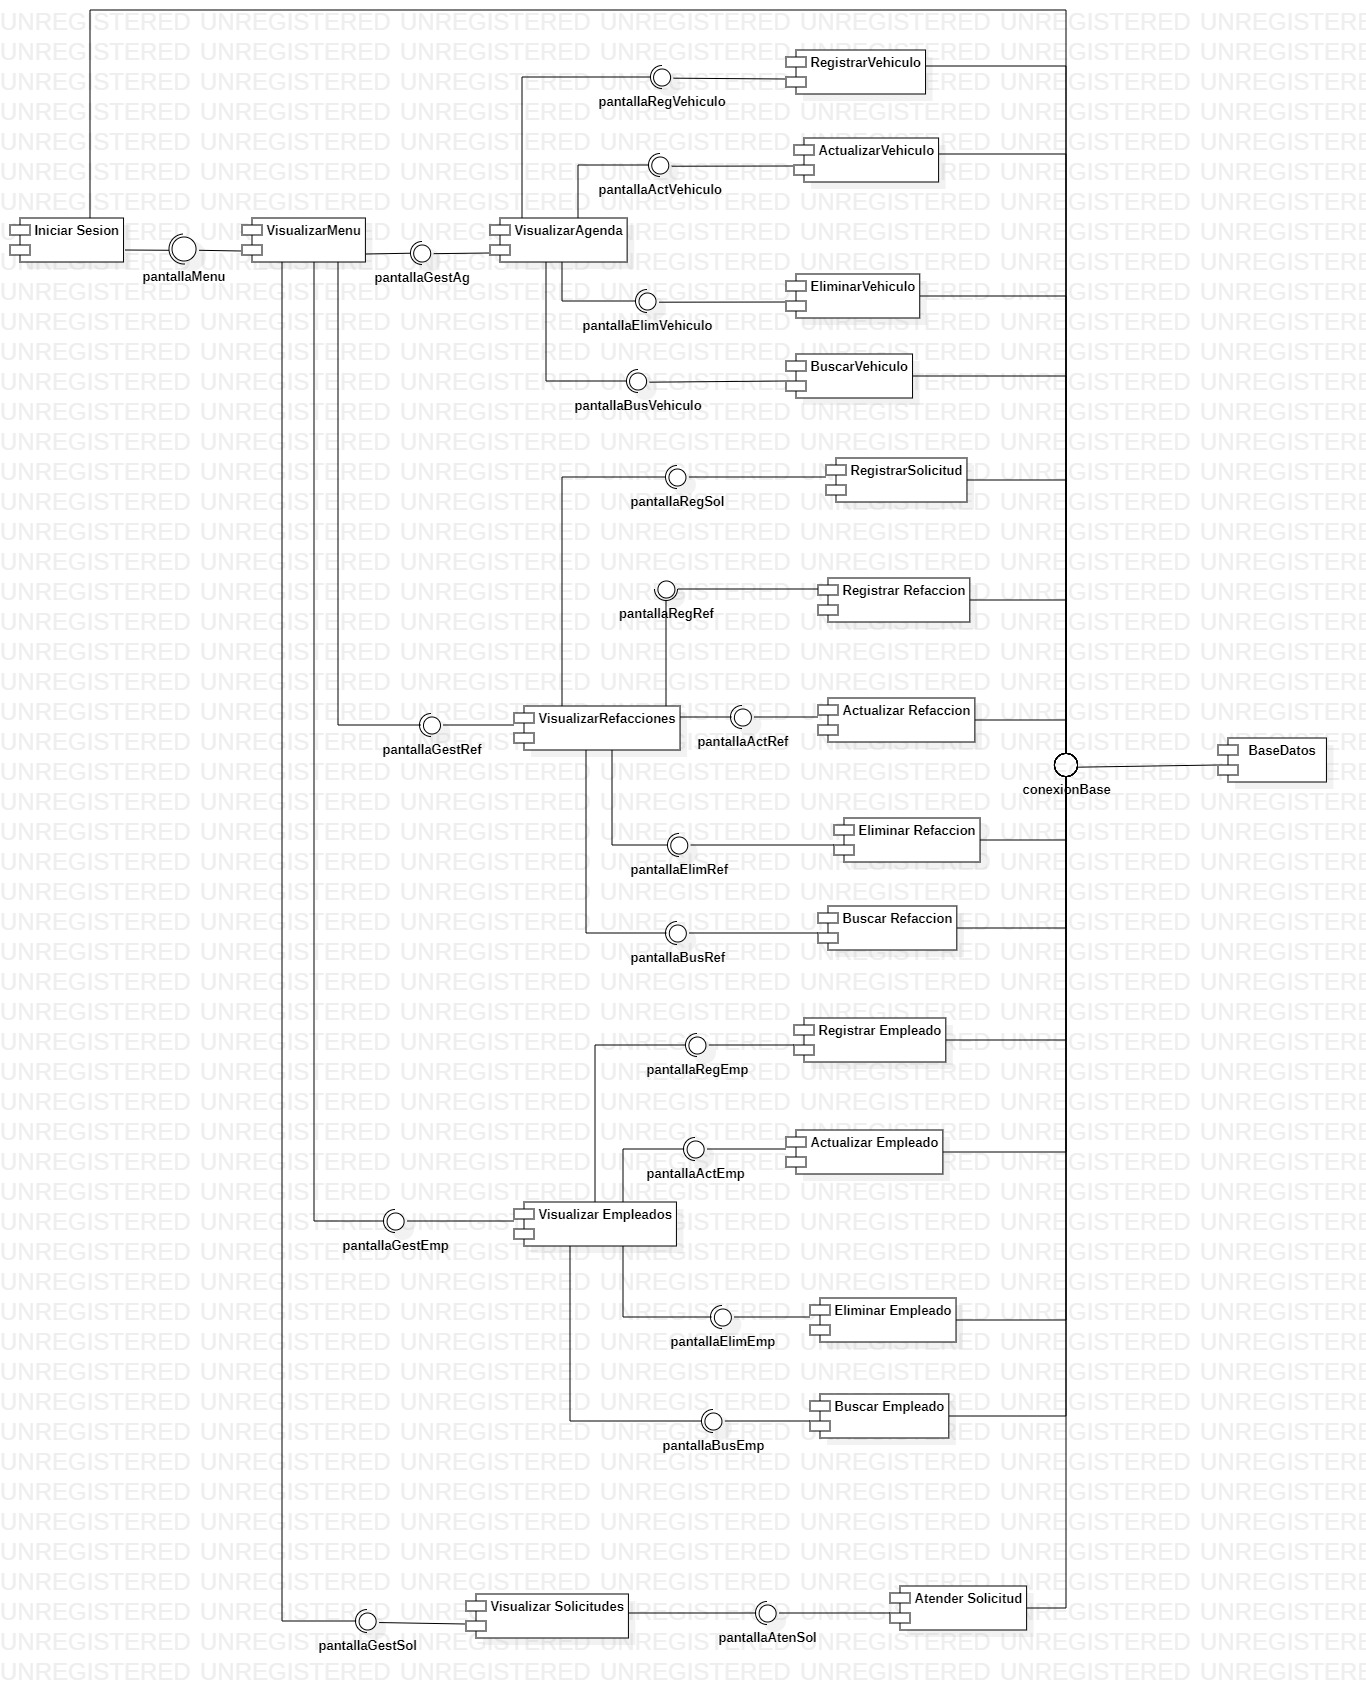
\includegraphics[width=1\textwidth]{./diseno/vdesarrollo/imagenes/vistaDesarrollo}
	\caption{Diagrama de Componentes - Vista de Desarrollo}
	\label{fig:Diagrama de Componentes - Vista de Desarrollo}
	\end{figure}
\clearpage